% \bibliography{../src/bibliography}

In this chapter I give background to this thesis.

\section{Syntax}
Introduce the background on syntax relevant for the chapters on parsing, and the syntactic evaluation. My aim is to provide a succinct and compelling answer to the inevitable question: \textit{Why do we care about constituency structure?} In particular I want to firmly establish the concept of constituents, and secondly I want to set some of the ground for the syntactic evaluation that we perform in the final chapter.
\begin{itemize}
  \item Introduce the central question: what are sentences, strings or structures? Is a sentence a string of words in linear order, or are the words combined in a hierarchical structure? \citep{everaert2015structures,frank2012hierarchical}
  \item The notion of a constituent, and constituent tests \citet{carnie2010constituent,huddleston2002grammar}.
  \item Hierarchical structure (of these constituents) \citet{everaert2015structures}.
  \item The lexical and phrasal categories of constituent analysis.
  \item Evidence for structured sentence processing from psycholinguistic research \citep{hale2001earley,levy2008expectation,brennan2016abstract}.
  \item Introduce the concept of \textit{acceptability judgements}, with the final chapter on syntactic evaluation in mind.
\end{itemize}

In the following exposition we primarily follow \citet{huddleston2002grammar}, with some excursions into \citet{carnie2010constituent} and \citet{everaert2015structures}. The first source is a well established reference grammar of the English language that is relatively agnostic with respect to theoretical framework, whereas the the later two sources are more firmly rooted in a particular framework\footnote{Broadly subsumable under the label \textit{generative grammar}.}. We take the following three pricinpiles (about English syntax!) from \citep{huddleston2002grammar} as guiding:
\begin{enumerate}[label=(\roman*)]
  \item Sentences consist of parts that may themselves have parts.
  \item These parts belong to a limited range of types.
  \item The constituents have specific roles in the larger parts they belong to.
\end{enumerate}

\paragraph{Constituents} Sentences consist of parts that may themselves have parts. The parts are groups of words that function as units, and they are called \textit{constituents}. Consider the simple sentence \textit{A bird hit the car.} The immediate constituents are \textit{a bird} (the subject) and \textit{hit the car} (the predicate). The phrase \textit{hit the car} can be further analyzed as containing the constituent \textit{the car}. The ultimate constituents of a sentence are the atomic words, and the entire analysis is called the constituent structure of the sentence. This structure can be indicated succinctly with the use of brackets
\begin{enumerate}
  \item [ [ A bird ] [ hit [ the car ] ] ]
  % \exig. [CP Heute [C$’$ scheint [TP [DP die Sonne ] [VP \I{t}V ]]\
  \label{eq:bird-brackets}
\end{enumerate}
or less succinctly as a tree as in figure \ref{fig:bird-tree}.
\begin{figure}[h]{\textwidth}
  \center
  \begin{tikzpicture}[scale=.8]
    \Tree [.$\cdot$ [.$\cdot$ A bird ] [.$\cdot$ hit [.$\cdot$ the car ] ] ]
  \end{tikzpicture}
  \caption{Sentence \ref{eq:bird-brackets} as a tree. (TODO: draw this without labels.)}
  \label{fig:bird-tree}
\end{figure}
Evidence for the existence of these constituents can be provided by examples such as the following, which are called constituent tests \citep{carnie2010constituent}. Consider inserting the adverb \textit{apparently} into our example sentence, indicating the alleged status of the event described in the sentence. In principle there are six positions available for the placement of \textit{apparently} (including before, and after the sentence). However, only three of these placements are actually permissible\footnote{We use an asterisk `*' to indicate a sentence that is judged ungrammatical, as is customary in linguistics.}:
\begin{enumerate}[noitemsep]
  \item \textit{Apparently} a bird hit the car.
  \item *An \textit{apparently} bird hit the car.
  \item A bird \textit{apparently} hit the car.
  \item *A bird hit \textit{apparently} the car.
  \item *A bird hit the \textit{apparently} car.
  \item A bird hit the car, \textit{apparently}.
\end{enumerate}
Based on the bracketing in \ref{eq:bird-brackets} we can formulate a general constraint: the adverb must not interrupt any constituent. Indeed, this explains why \textit{actually} cannot be placed anywhere inside \textit{hit the car} and not between \textit{a} and \textit{bird}. For full support, typically results from many more such test are gathered, and in general these tests can be much more controversial than in our simple example \citep{carnie2010constituent}.

\paragraph{Syntactic categories} The constituents of a sentence belong to a limited range of types that form the set of syntactic categories \citep{huddleston2002grammar}. Two types are distinguished: lexical categories (part of speech) and phrasal categories. The tree in figure \ref{fig:bird-tree} can be represented in more detail by adding syntactic categories, see figure \ref{fig:bird-tree-labeled}.
\begin{figure}[h]{\textwidth}
  \center
  \begin{tikzpicture}[scale=.8]
    \Tree [.S [.NP [.D A ] [.N bird ]] [.VP [.V hit ] [.NP [.D the ] [.N car ] ] ] ]
  \end{tikzpicture}
  \caption{A tee specified with lexical (D, N, V) and phrasal categories (S, NP, VP).}
  \label{fig:bird-tree-labeled}
\end{figure}

\begin{figure}[b]
  \begin{subfigure}[b]{0.5\textwidth}
		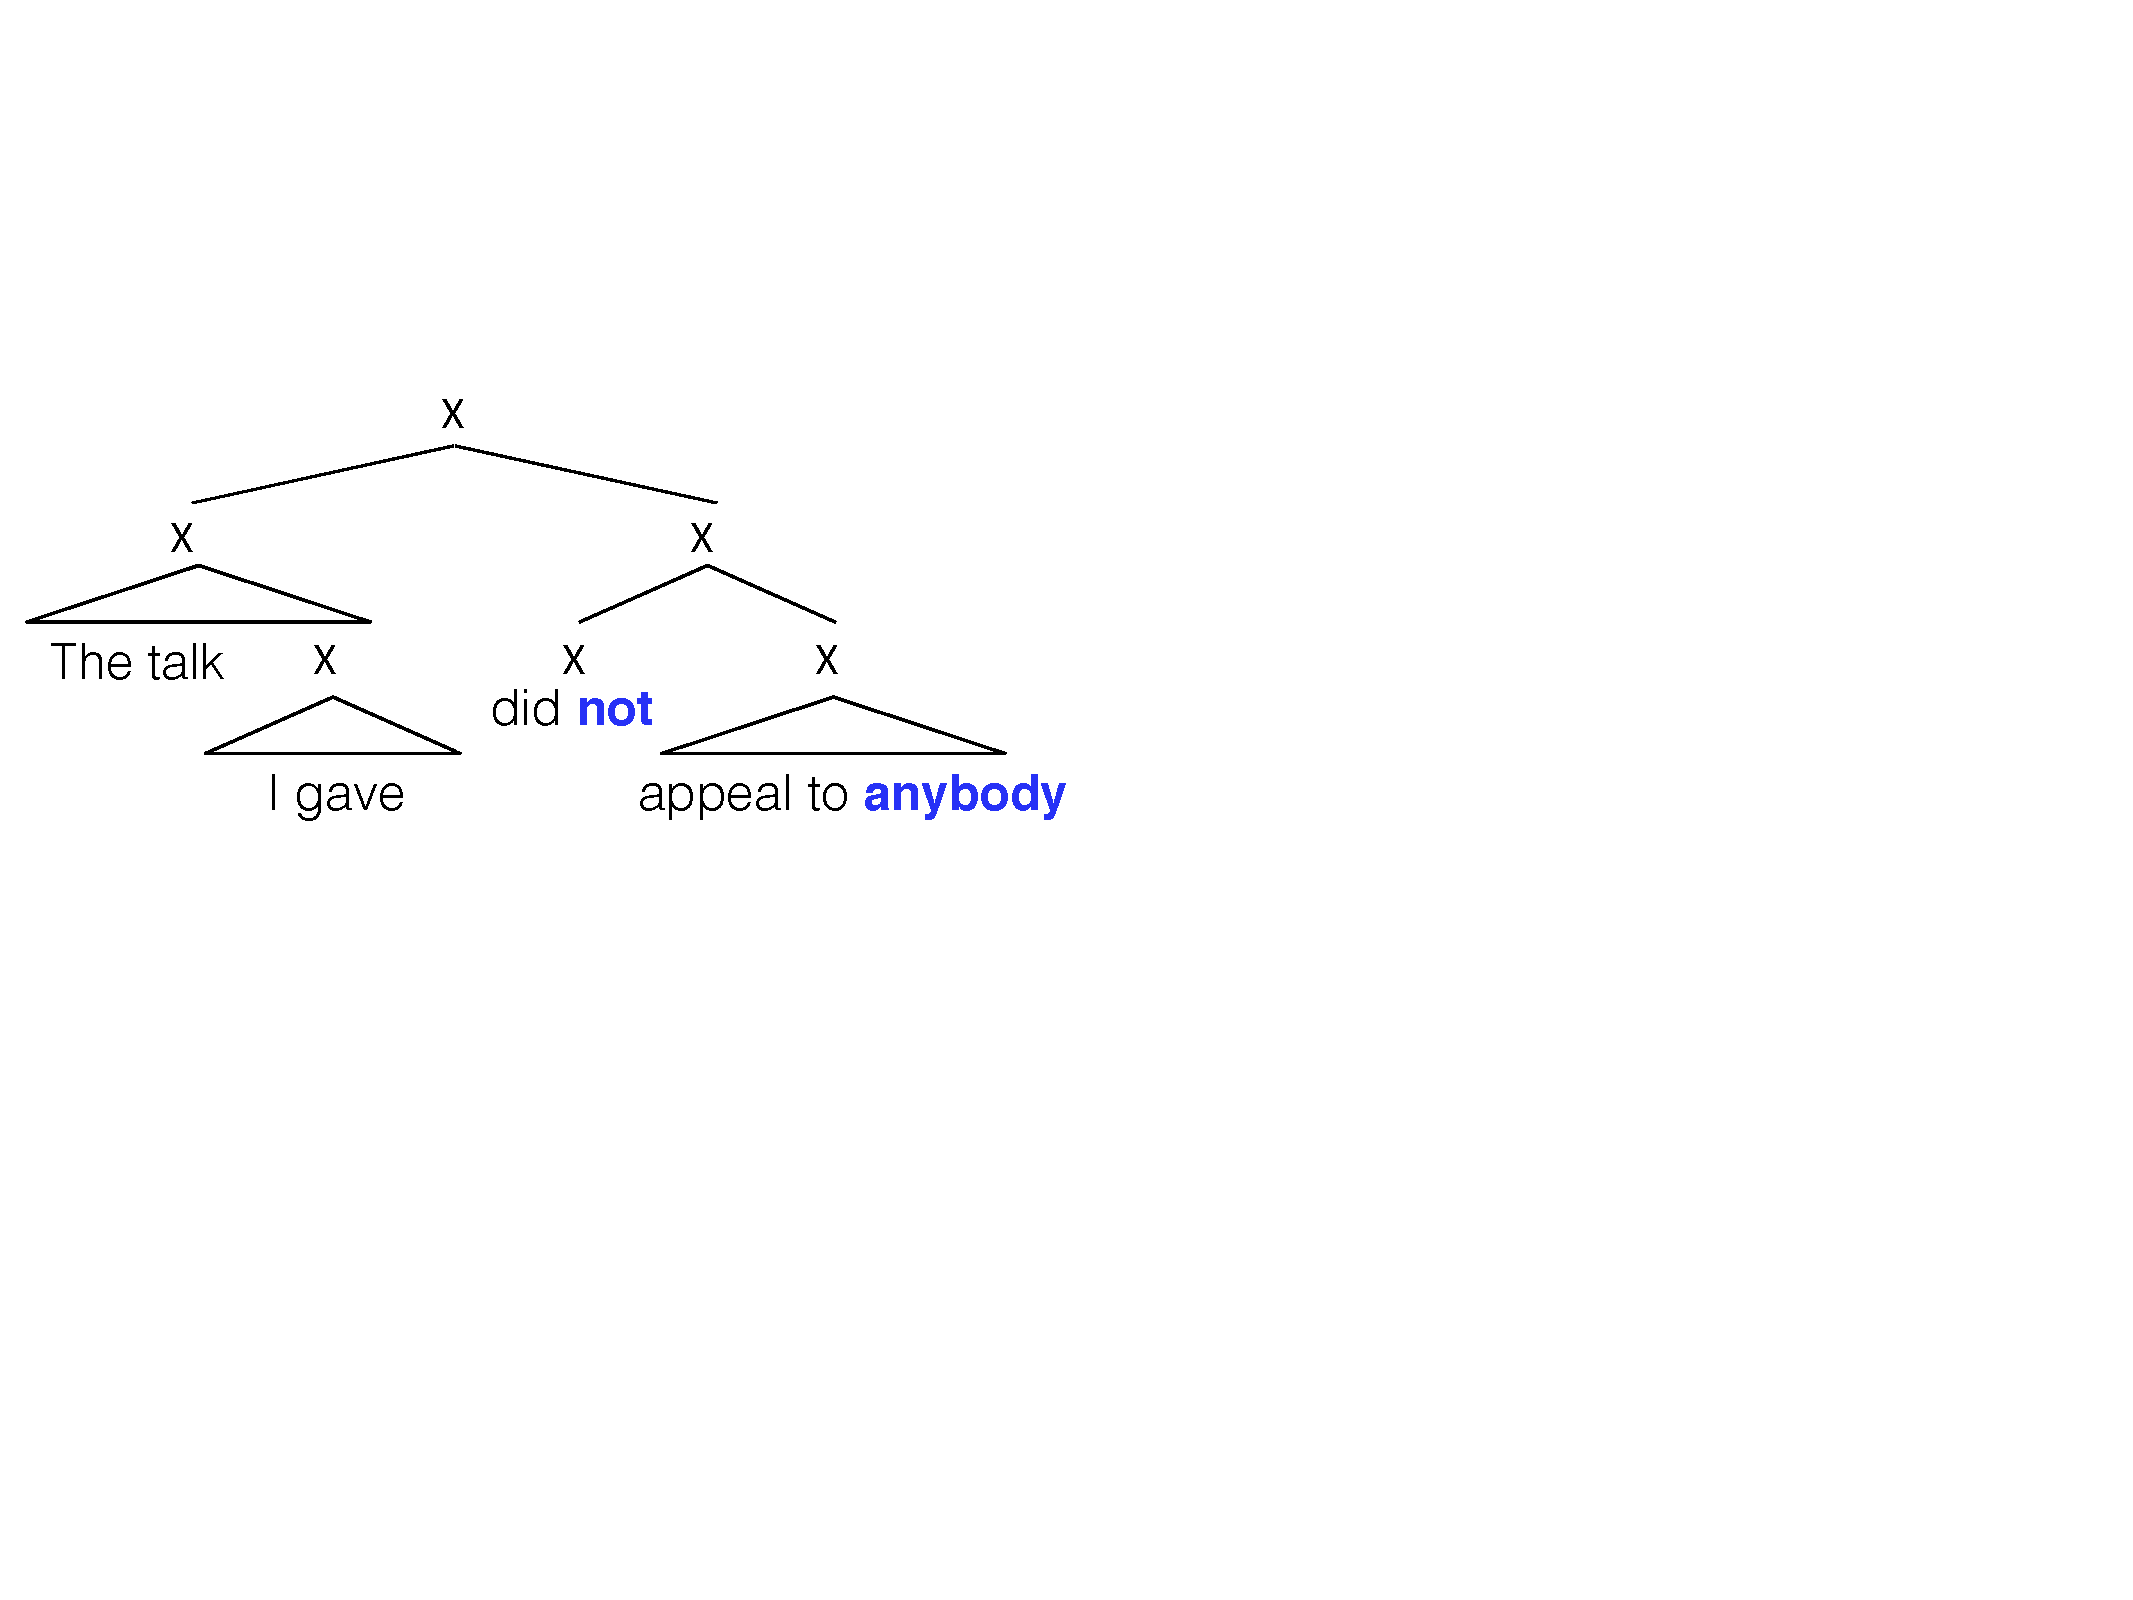
\includegraphics[width=0.9\textwidth]{trees/npi-licensed.pdf}
    \label{fig:tree-npi-licensed}
    \subcaption{In licensing context.}
	\end{subfigure}
	\begin{subfigure}[b]{0.5\textwidth}
		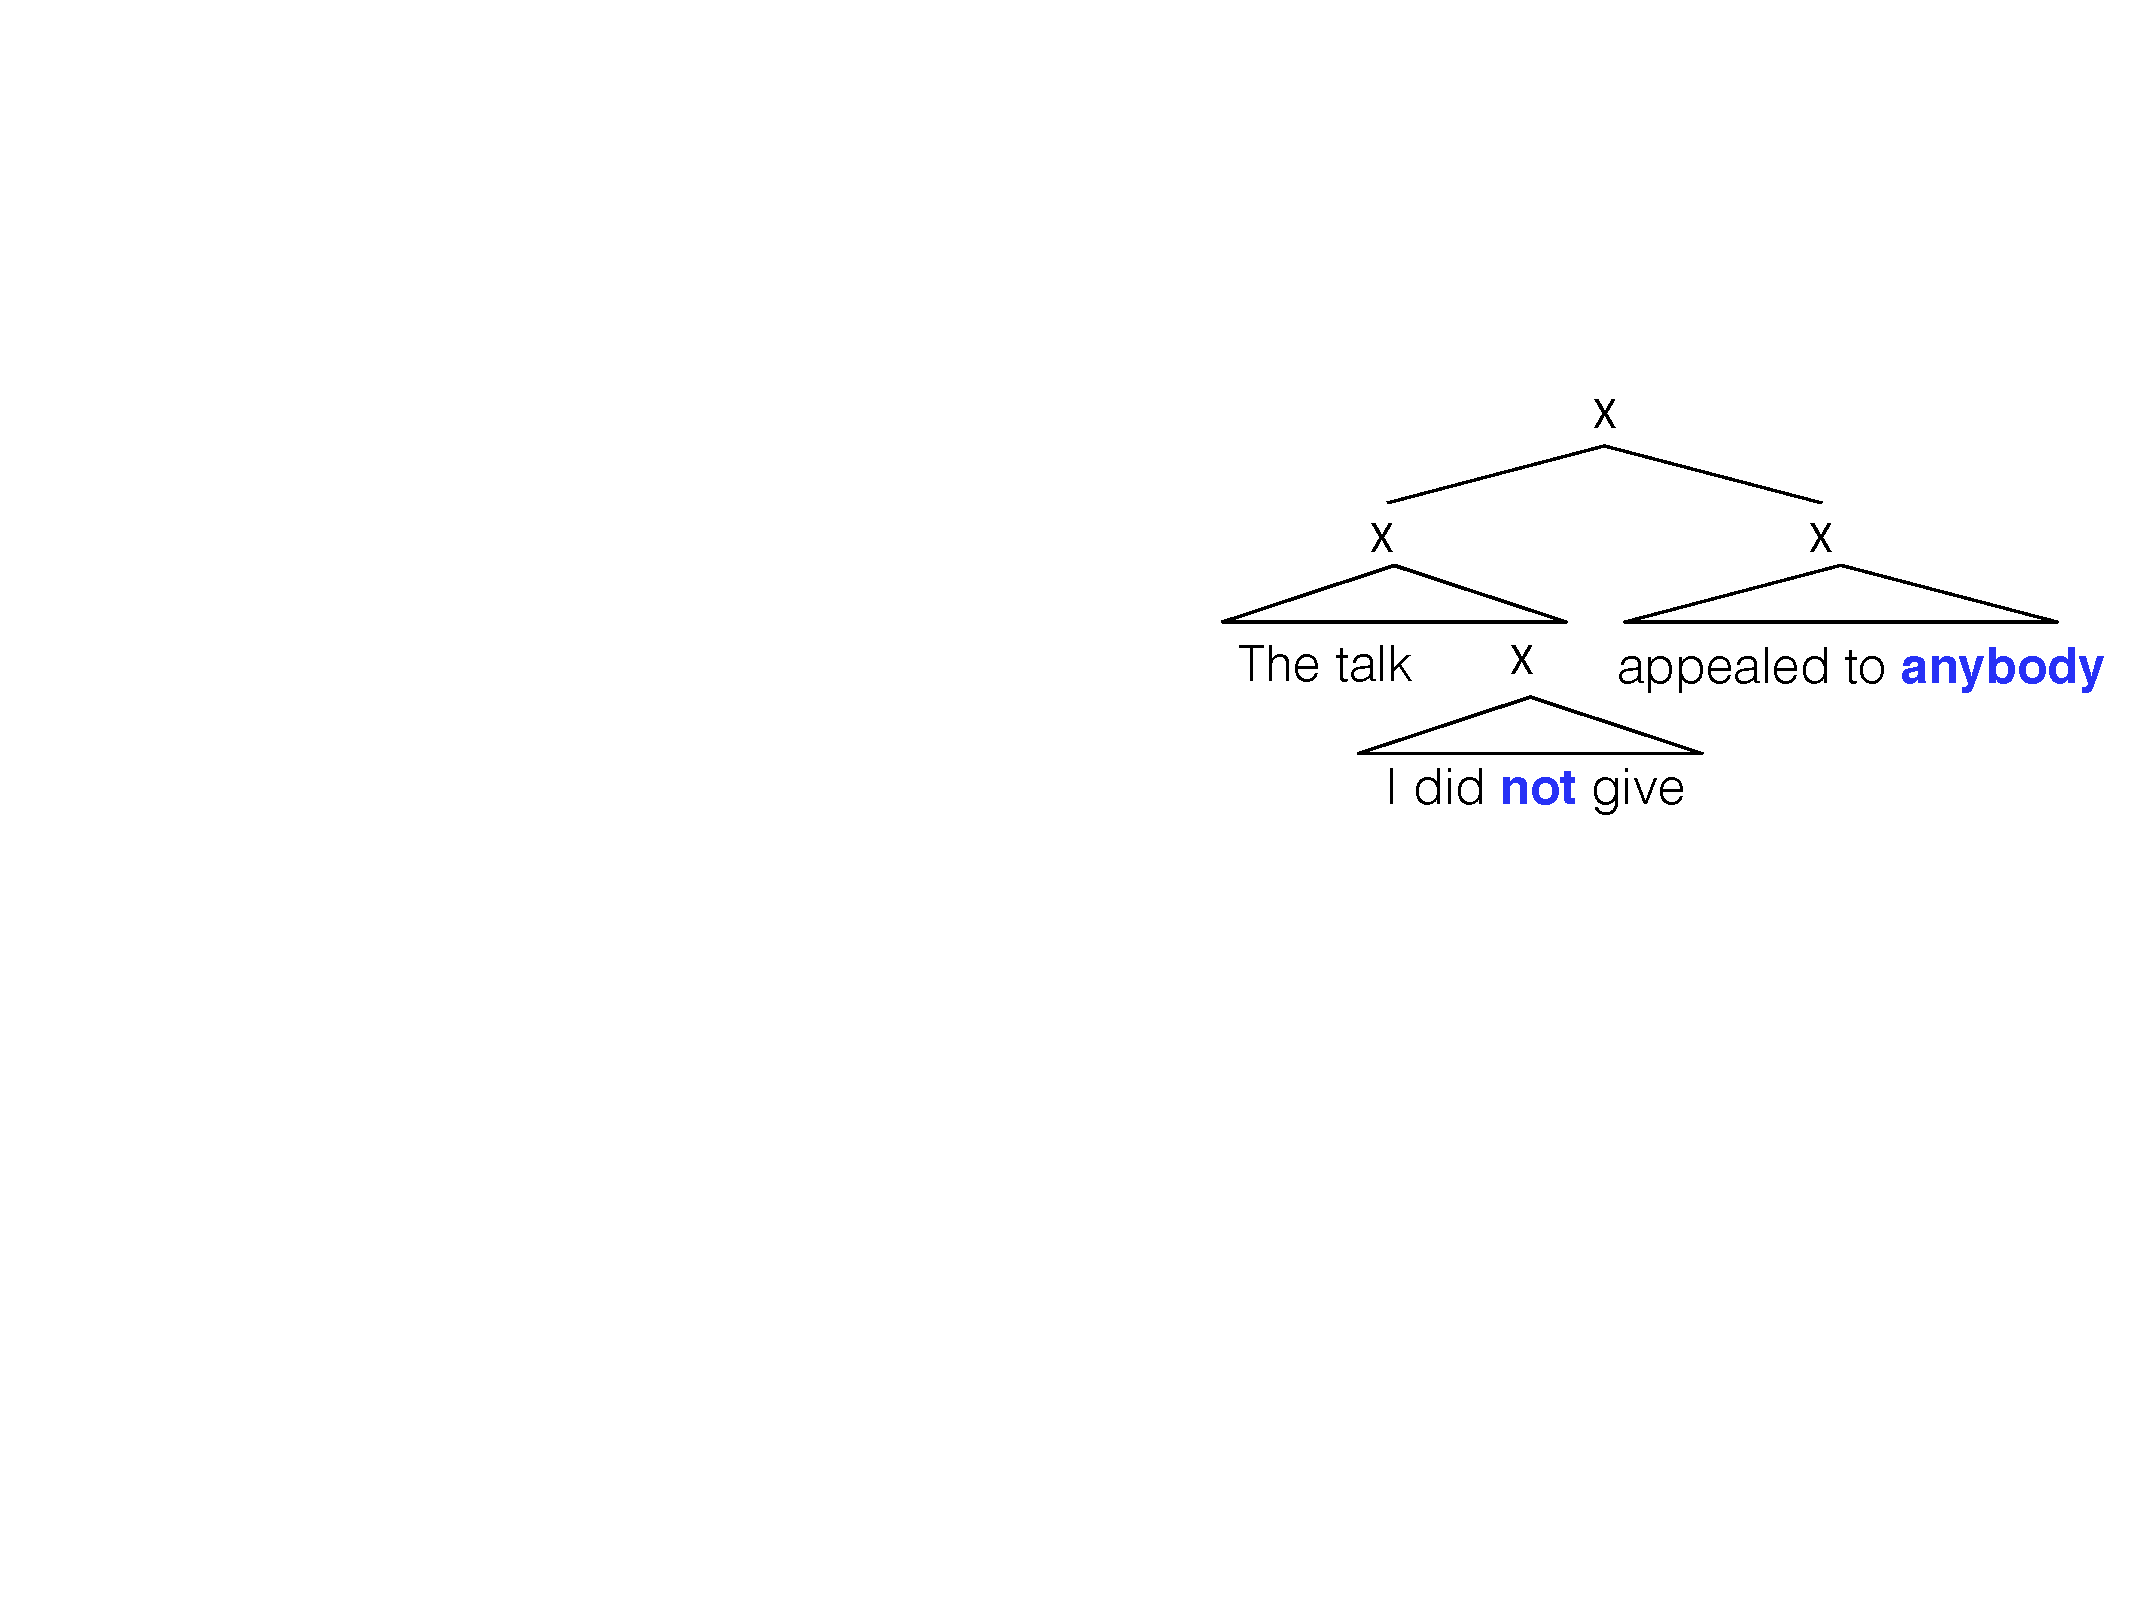
\includegraphics[width=0.9\textwidth]{trees/npi-unlicensed.pdf}
    \label{fig:tree-npi-unlicensed}
    \subcaption{Not in licensing context.}
	\end{subfigure}
\caption{Negative Polarity. Figure taken from \cite{everaert2015structures}. (TODO: draw in qtree, but how to make the nested roofs?)}
\label{fig:trees-npi}
\end{figure}

\paragraph{Hierarchical structure} The constituents have specific roles in the larger parts they belong to \citep{huddleston2002grammar}. This structure provides constraints that are not explainable from the linear order of the words themselves. Consider the following example about the syntactic behaviour of \textit{negative polarity items} (NPIs)\footnote{A negative polarity item is, to first approximation, a word or group of words that is restricted to negative context \citep{everaert2015structures}. More generaly they are words that need to be licensed by a specific \textit{licencing context} \citep{giannakidou2011npi}.} such as \textit{anybody}:
\begin{enumerate}[noitemsep]
  \item The book that I bought did \textit{not} appeal to \textit{anybody}.
  \item * The book that I bought appealed to \textit{anybody}.
\end{enumerate}
From this example we might formulate the hypothesis that the word \textit{not} must linearly precede the word \textit{anybody}. A counter example refutes this linear hypothesis:
\begin{enumerate}
  \item *The book I did \textit{not} buy appealed to \textit{anybody}.
\end{enumerate}
Instead, the constraints that govern this particular pattern depend on hierarchical structure: the word \textit{not} must ``structurally precede'' the word \textit{anybody} \citep{everaert2015structures}. Figure \label{ref:trees-npi} shows the constituent structure of both sentences. The explanation goes as follows (put this in my own words): \say{In sentence \ref{fig:trees-npi} (a) the hierarchical structure dominating \textit{not} also immediately dominates the hierarchical structure containing \textit{anybody}. In sentence \ref{fig:trees-npi} (b), by contrast, \textit{not} sequentially precedes \textit{anybody}, but the triangle dominating \textit{not} fails to also dominate the structure containing \textit{anybody}.}

\paragraph{Cognitive reality} Does all this exist in the human brain? These people say \textit{yes}: \citep{hale2001earley,levy2008expectation,brennan2016abstract}.

\paragraph{Controversy}
Theoretical syntax is rife with controversy, and wildly differing viewpoints exist. In fact, for each point made in our short discussion, the exact opposite point has been made as well:
\begin{itemize}
  \item Constituents are fundamental \citep{huddleston2002grammar,carnie2010constituent} \textit{versus} word-word relations are all you need \citep{tesniere1959elements,nivre2005dependency,hudson2010introduction}.
  \item Hierarchical structure is a core feature of language \citep{everaert2015structures} \textit{versus} sequential sentence structure has enough explanatory power \cite{frank2012hierarchical}. The claim is that (2) is cognitively more fundamental than (1),
  \begin{enumerate}
    \item [Sentences [ [can [be analysed] ] [as [hierarchically structured] ] ] ]
    \item [Sentences] [can be analysed] [as hierarchically structured]
  \end{enumerate}
  which is exactly contrary to the analyses above. This is more similar to the NLP task of \textit{chunking}, or shallow parsing.
  \item Studies in cognitive neuroscience and psycholinguistics show that human sentence processing is hierachical \citep{hale2001earley,levy2008expectation,brennan2016abstract} \textit{and} they show that it is not \citep{conway2008neurocognitive,christiansen2012similar,gillespie2011hierarchy, gillespie2013against} (selected from the survey in \citet{frank2012hierarchical}).
\end{itemize}
In this research I take a position of extreme pragmatism with respect to syntax: it is whatever our dataset says it is. Which means in our case, the Penn Treebank has the final word on the subject. And is language hierachical or linear? That is exactly what we inted to ivestigate from a statistical and computational viewpoint.

% \begin{figure}
%   \begin{subfigure}[b]{\textwidth}
%     \center
%     \begin{tikzpicture}[scale=.6]
% 		  \setbox\partbox=\hbox{\qroof{that I bought}.X }

\Tree [.X
        \qroof{The book \usebox{\partbox}}.X
        [.X
          \qroof{did \textit{not}}.X
          \qroof{appeal to \textit{anybody}}.X ]]

% \Tree [.X
%         [.X
%           The book \edge[roof]; { that I bought } ]
%         [.X
%           [.X \edge[roof]; {did \textit{not}} ]
%           [.X \edge[roof]; {appeal to \textit{anybody}} ] ] ]

%     \end{tikzpicture}
% 		\label{fig:tree-npi-licensed}
%   \end{subfigure}
%
%   \begin{subfigure}[b]{\textwidth}
%     \center
%     \begin{tikzpicture}[scale=.6]
% 		  \Tree [.X
        [.X
          The book \edge[roof]; { that I did \textit{not} buy } ]
        [.X
          [.X \edge[roof]; {did \textit{not}} ]
          [.X \edge[roof]; {appeal to \textit{anybody}} ] ] ]

%     \end{tikzpicture}
% 		\label{fig:tree-npi-unlicenced}
%   \end{subfigure}
%
% \caption{Negative Polarity.}
% \label{fig:trees-npi}
% \end{figure}


\section{Parsing}
\begin{itemize}
  \item Treebanks, in particular the Penn Treebank. Treebank preprocessing. CFGs, CNF, spans. Reference figure \ref{fig:trees-ptb}.
  \item The two conceptions of a tree: as a set of \textit{labeled spans} or as a set of \textit{anchored rules}.
  \item A labeled span is a triple $(\ell, i, j)$ of a syntactic label $\ell$ together the left and right endpoints $i$, $j$ that the label spans.
  \item An \textit{anchored rule} is a triple $(r, i, j)$ or four-tuple $(r, i, k, j)$, containing a CNF rule $r$ with span endpoints $i$, $j$, and a split-point $k$ of the left and right child $r$ is not a lexical rule.
  \item For the difference, consider the following two representations of the tree in figure \ref{fig:tree-cnf-spans} given in table \ref{tab:spans-rules}.
  \item Algorithms for parsing: global chart based, local transition based
  \item Dynamic programming inference versus search heuristics.
  \item Modelling types: generative, discriminative, log-linear, count-based, feature-based, neural network features.
\end{itemize}

% As images.
% \begin{figure}
% 	\centering
%   \begin{subfigure}{0.72\textwidth}
% 		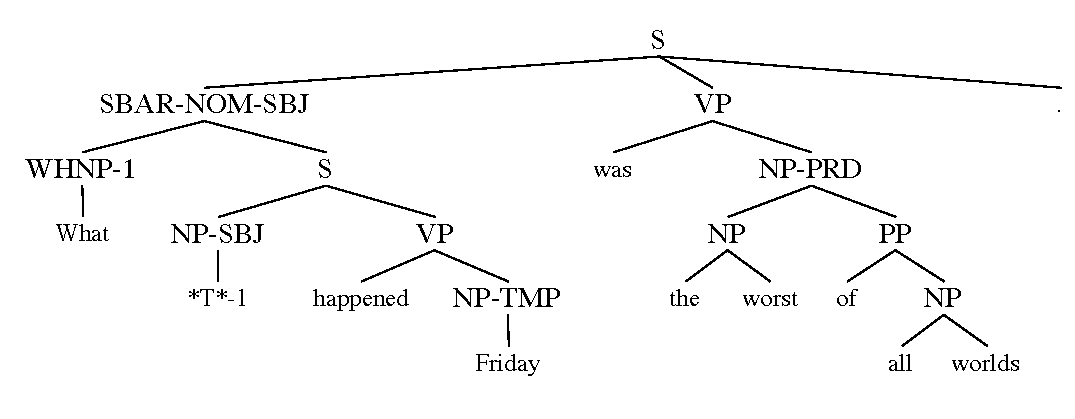
\includegraphics[width=\textwidth]{trees/original.pdf}
%     \caption{Original Penn Treebank tree.}
% 		\label{fig:tree-original}
% 	\end{subfigure}
% 	\begin{subfigure}{0.62\textwidth}
% 		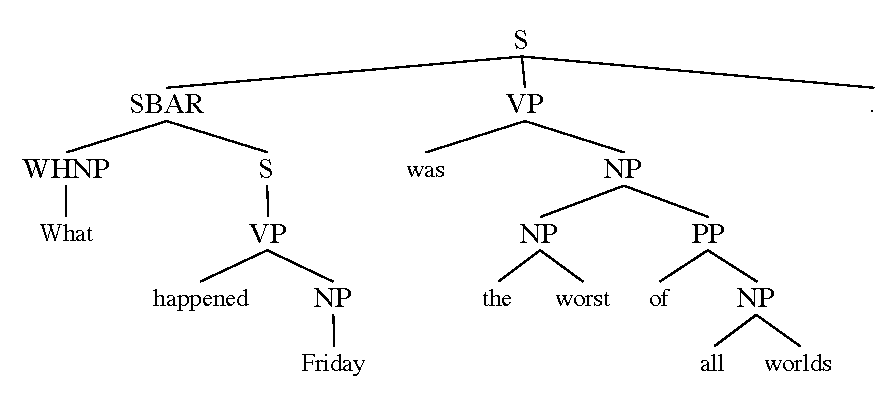
\includegraphics[width=\textwidth]{trees/simplified.pdf}
%     \caption{Function tags and traces removed.}
% 		\label{fig:tree-simplified}
% 	\end{subfigure}
% 	\begin{subfigure}{0.62\textwidth}
% 		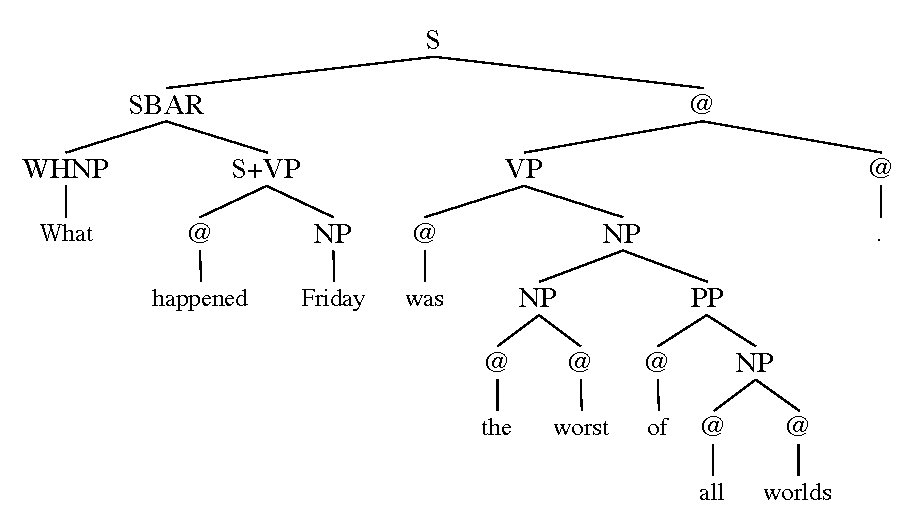
\includegraphics[width=\textwidth]{trees/binary.pdf}
%     \caption{Converted to normal form.}
% 		\label{fig:tree-cnf}
% 	\end{subfigure}
% 	\begin{subfigure}{0.9\textwidth}
% 		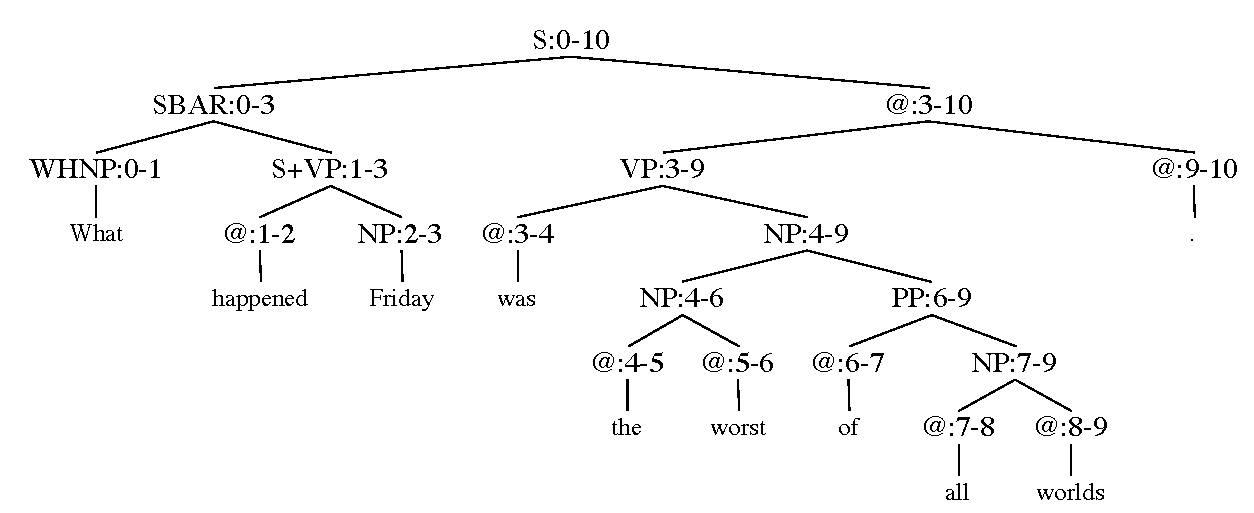
\includegraphics[width=\textwidth]{trees/spans.pdf}
%     \caption{In normal form with spans.}
% 		\label{fig:tree-cnf-spans}
% 	\end{subfigure}
%   \caption{Converting a treebank tree (withouth part-of-speech tags).}
%   \label{fig:trees-ptb}
% \end{figure}

\begin{figure}

  \begin{subfigure}[b]{\textwidth}
    \center
    \begin{tikzpicture}[scale=.6]
      \Tree [.S
        [.SBAR-NOM-SBJ
          [.WHNP-1 What ]
          [.S [.NP-SBJ *T*-1 ] [.VP happened [.NP-TMP Friday ] ] ] ]
        [.VP
          was
          [.NP-PRD [.NP the worst ] [.PP of [.NP all worlds ] ] ] ]
        . ]

    \end{tikzpicture}
    \subcaption{Original Penn Treebank tree.}
		\label{fig:tree-original}
  \end{subfigure}

  \begin{subfigure}[b]{\textwidth}
    \center
    \begin{tikzpicture}[scale=.6]
		  \Tree [.S
        [.SBAR [.WHNP What ] [.S [.VP happened [.NP Friday ] ] ] ]
        [.VP
          was
          [.NP [.NP the worst ] [.PP of [.NP all worlds ] ] ] ]
        $.$ ]

    \end{tikzpicture}
    \tiny
    \subcaption{Function tags and traces removed.}
		\label{fig:tree-simplified}
  \end{subfigure}

  \begin{subfigure}[b]{\textwidth}
    \center
    \begin{tikzpicture}[scale=.6]
		  \Tree [.S
        [.SBAR [.WHNP What ] [.S+VP [.$\varnothing$ happened ] [.NP Friday ] ] ]
        [.$\varnothing$
          [.VP
            [.$\varnothing$ was ]
            [.NP
              [.NP [.$\varnothing$ the ] [.$\varnothing$ worst ] ]
              [.PP [.$\varnothing$ of ] [.NP [.$\varnothing$ all ] [.$\varnothing$ worlds ] ] ] ] ]
          [.$\varnothing$ . ] ] ]

    \end{tikzpicture}
    \tiny
    \subcaption{Converted to normal form.}
		\label{fig:tree-cnf}
  \end{subfigure}

  \begin{subfigure}[b]{\textwidth}
    \center
    \begin{tikzpicture}[scale=.6]
		  \Tree [.S:0-10
        [.SBAR:0-3
          [.WHNP:0-1 What ]
          [.S+VP:1-3 [.@:1-2 happened ] [.NP:2-3 Friday ] ] ]
        [.@:3-10
          [.VP:3-9
            [.@:3-4 was ]
            [.NP:4-9
              [.NP:4-6 [.@:4-5 the ] [.@:5-6 worst ] ]
              [.PP:6-9
                [.@:6-7 of ]
                [.NP:7-9 [.@:7-8 all ] [.@:8-9 worlds ] ] ] ] ]
          [.@:9-10 . ] ] ]

    \end{tikzpicture}
    \tiny
    \subcaption{In normal form with spans.}
		\label{fig:tree-cnf-spans}
  \end{subfigure}

\caption{Converting a treebank tree (withouth part-of-speech tags).}
\label{fig:trees-ptb}
\end{figure}


\begin{table}[h]
  \center
  \small
  \bgroup  % increase vertical space
  \def\arraystretch{1.5}  % increase vertical space
  \begin{tabular}{l|l}
    Labeled spans & Anchored rules \\
    \hline
    (S, 0, 10)     & (S $\to$ SBAR $\varnothing$, 0, 3, 10)  \\
    (SBAR, 0, 3)   & (SBAR $\to$ WHNP S+VP, 0, 1, 3)  \\
    % (VP, 1, 3)     & (S+VP $\to$ $\varnothing$ NP, 1, 2, 3)  \\
    (WHNP, 0, 1)     & (WHNP $\to$ \textit{What}, 0, 1)  \\
    $\qquad\vdots$ & $\qquad\vdots$  \\
    % (NP, 7, 9)     & (NP $\to$ $\varnothing$ $\varnothing$, 7, 8, 9)  \\
    ($\varnothing$, 9, 10)     & ($\varnothing$ $\to$ ., 9, 10)  \\
  \end{tabular}
  \caption{Two conceptions of the tree in \ref{fig:tree-cnf-spans}.}
  \label{tab:spans-rules}
  \egroup  % increase vertical space
\end{table}


\section{Language models}
\begin{itemize}
  \item Briefly mention some typical approaches for langugage modelling: count based n-gram with smoothing \citep{chen1999empirical,kneser1995improved}, neural n-gram \citep{bengio2003neural} and recurrent neural network \citep{mikolov2010recurrent}. Also mention some (early) syntactic approaches: count-based \citep{chelba2000structured,pauls2012treelets}, neural \citep{emami2005neural}, and top-down parsing related \citep{roark2001probabilistic}.
  \item Explain the metric perplexity.
  \item Briefly mentions some typical datasets and some benchmarks (dataset, perplexity, number of parameters, training time).
  \item Mention some downsides of the perplexity metric: conflating different sources of succes in next-word prediction (simple collocations, semantics, syntax).
  \item Note that there exists some alternatives to perplexity: adversarial evaluation \citep{smith2012adversarial}, subject-verb agreement \citep{linzen2016syntax} and grammatical acceptability judgments \citep{linzen2018targeted}.
\end{itemize}


\section{Neural networks}
Introduce all the neural networks.
\begin{itemize}
  \item We consider the neural networks as abstractions denoting certain parametrized functions \ff, \rnn, \lstm, etc.
  \item Let $\x$ and $\y$ be vectors in respectively $\reals^{n}$ and $\reals^{m}$.

  A \textit{feedforward neural network} is a parametrized function $\ff$ from $\reals^{n}$ to $\reals^{m}$ such that
  \begin{align*}
    \ff( \x ) &= \y.
  \end{align*}

  A \textit{recurrent neural network} is a parametrized function \rnn that takes a sequence of vectors $(\x_i)_{i=1}^n = ( \x_1, \x_2, \dots, \x_n )$ in $\reals^{n}$ and produces a sequence of output vectors in $( \y_1, \y_2, \dots,\y_n )$ in $\reals^{m}$:
  \begin{align*}
    \rnn( (\x_i)_{i=1}^n ) &= ( \y_1, \y_2, \dots, \y_n ).
  \end{align*}
  Internally, the \rnn recursively applies a function $f: \reals^{n} \times \reals^{m} \to \reals^{m}$ that is defined by the recursion
  \begin{align*}
    \y_{t} &= f(\x_t, \y_{t-1})  \\
      &= f(\x_t, f(\x_{t-1}, \y_{t-2}))  \\
      &\;\vdots \\
      &= f(\x_t, f(\x_{t-1}, f(\dots f(\x_{1}, \y_{0})))),
  \end{align*}
  which is how the vectors $\y_i$ are computed. That is, $f$ takes the input $\x$ of the current timestep $t$ and the output $\y$ of the previous timestep $t-1$ and returns a new ouput for timestep $t$. The initial vector $\y_{0}$ does not depend on the input, and can be fixed or part of the function's set of parameters.

  An \rnn can be applied to the input sequence in reverse, that is, in the \textit{backward} direction:
  \begin{align*}
    \rnn_B( (\x_i)_{i=1}^n )
      &= \rev( \rnn( \rev( (\x_i)_{i=1}^n ) ) ) \\
      &= \rev( \rnn( \x_n, \x_{n-1}, \dots, \x_1 ) \\
      &= \rev( \y_n, \y_{n-1}, \dots, \y_1 ) \\
      &= (\y_1,\y_2, \dots, \y_n ), \\
  \end{align*}
  where we defined a
  \begin{equation}
    \rev( (\x_i)_{i=1}^n ) \defeq ( \x_n, \x_{n-1}, \dots, \x_1 ),
  \end{equation}

  For consistency we will refer to the \rnn in the regular, \textit{forward}, direction as $\rnn_F$. To stress the difference between the different outputs obtained from the two directions, we will denote the output vectors obtained in the regular, forward, direction with $\fw_i$ and the vectors obtained in the backward direction with $\bw_i$:
  \begin{align*}
    \rnn_F( (\x_i)_{i=1}^n ) &= ( \fw_1, \fw_2, \dots, \fw_n ) \\
    \rnn_B( (\x_i)_{i=1}^n ) &= ( \bw_1, \bw_2, \dots, \bw_n )
  \end{align*}
  The two functions above can used to construct a \textit{bidirectional} \rnn by combining the output of each as
  \begin{equation}
    \birnn( (\x_i)_{i=1}^n ) = ( \fw_1 \concat \bw_1, \fw_2 \concat \bw_2, \dots, \fw_n \concat \bw_n ),
  \end{equation}
  where we use $\concat$ to denote vector concatenation, \ie $\x \concat \y$ is a vector in $\reals^{n+m}$.

  An \lstm is a particular way to construct the \rnn internal function $f$, and similarly has a bidirectional equivalent denoted \bilstm.
  \item The function \ff is defined as follows:
  \item The function \lstm is defined as follows
  \item (Minibatch) SGD optimization.
\end{itemize}
